\documentclass[aspectratio=169]{beamer}

\usetheme{Madrid}
\setbeamertemplate{navigation symbols}{}
\setbeamertemplate{footline}[frame number]

\usepackage[utf8]{inputenc}
\usepackage{graphicx}
\usepackage{listings}
\usepackage{xcolor}
\usepackage{booktabs}
\usepackage{tikz}
\usetikzlibrary{positioning}

\definecolor{mongogreen}{RGB}{0,104,74}
\definecolor{primary}{RGB}{0,140,80}
\definecolor{secondary}{RGB}{30,100,200}
\definecolor{orange}{RGB}{220,110,20}
\definecolor{danger}{RGB}{190,40,40}
\definecolor{codebg}{RGB}{245,245,245}

\setbeamercolor{frametitle}{bg=mongogreen, fg=white}
\setbeamercolor{structure}{fg=mongogreen}
\setbeamercolor{block title}{bg=mongogreen, fg=white}
\setbeamercolor{block body}{bg=gray!10, fg=black}
\setbeamercolor{alerted text}{fg=danger}
\setbeamercolor{footline}{fg=black, bg=gray!15}

\lstset{
  basicstyle=\ttfamily\tiny,
  backgroundcolor=\color{codebg},
  keywordstyle=\color{primary},
  stringstyle=\color{orange},
  commentstyle=\color{gray!60!black},
  frame=single,
  rulecolor=\color{gray!40},
  breaklines=true,
  showstringspaces=false
}

\title[CENG465]{Data Replication in a Single-Leader Environment}
\subtitle{MongoDB Replica Set + Python Control Node}
\author{Mert Karahan \and Do\u{g}ukan Top\c{c}u}
\institute{CENG465 --- Principles of Data-Intensive Systems}
\date{May 5, 2026}

\begin{document}

% ── 1: Title ──────────────────────────────────────────────────────────────────
\begin{frame}
  \titlepage
\end{frame}

% ── 2: Project Overview ───────────────────────────────────────────────────────
\begin{frame}{Project Overview}
  \begin{columns}
    \column{0.52\textwidth}
      \small\textbf{Goal:} demonstrate single-leader replication on two physical macOS machines — no containers, real LAN.
      \begin{itemize}\small
        \item MongoDB \texttt{rs0} replica set (PRIMARY + SECONDARY)
        \item Schema with version, log-index, and operation-id tracking
        \item Python/Flask control node \& live dashboard
        \item Write concern toggle: \texttt{w=majority} vs \texttt{w=1}
        \item Background reconciler for async catch-up detection
      \end{itemize}
    \column{0.44\textwidth}
      \begin{block}{Core question}
        \small What happens when the follower goes offline?
        \begin{itemize}\small
          \item \texttt{w=majority}: reject the write
          \item \texttt{w=1}: accept the write, queue it
          \item How do we \textbf{observe} catch-up?
        \end{itemize}
      \end{block}
      \begin{block}{Machines}
        \small
        \begin{tabular}{ll}
          Primary   & \texttt{192.168.88.146} \\
          Secondary & \texttt{192.168.88.105} \\
        \end{tabular}
      \end{block}
  \end{columns}
\end{frame}

% ── 3: Deployment Architecture ────────────────────────────────────────────────
\begin{frame}{Deployment Architecture}
  \begin{center}
  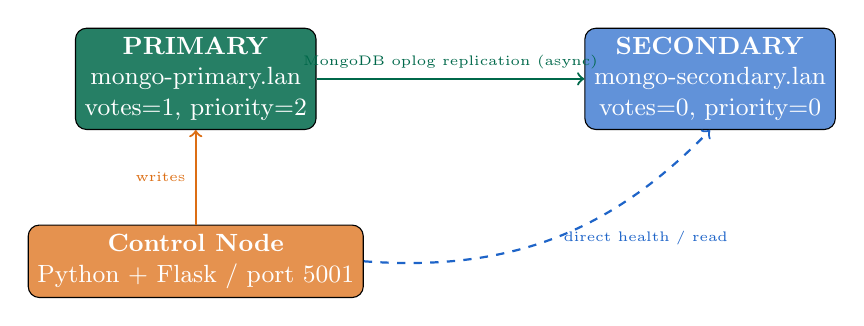
\begin{tikzpicture}[
    node distance=1.6cm,
    box/.style={draw, rounded corners, minimum width=2.8cm, minimum height=0.85cm, align=center, font=\small},
    arrow/.style={->, thick}
  ]
    \node[box, fill=mongogreen!85, text=white] (prim) {\textbf{PRIMARY}\\mongo-primary.lan\\votes=1, priority=2};
    \node[box, fill=secondary!70, text=white, right=3.4cm of prim] (sec) {\textbf{SECONDARY}\\mongo-secondary.lan\\votes=0, priority=0};
    \node[box, fill=orange!75, text=white, below=1.2cm of prim] (ctrl) {\textbf{Control Node}\\Python + Flask / port 5001};
    \draw[arrow, color=mongogreen] (prim) -- node[above, font=\tiny]{MongoDB oplog replication (async)} (sec);
    \draw[arrow, color=orange] (ctrl) -- node[left, font=\tiny]{writes} (prim);
    \draw[arrow, color=secondary, dashed] (ctrl.east) to[bend right=25] node[right, font=\tiny]{direct health / read} (sec.south);
  \end{tikzpicture}
  \end{center}
  \begin{columns}
    \column{0.48\textwidth}
      \begin{block}{Why non-voting secondary?}
        \footnotesize With two voting members, disconnecting secondary removes majority — primary steps down and even \texttt{w=1} cannot write. \texttt{votes=0} keeps primary writable during outages.
      \end{block}
    \column{0.48\textwidth}
      \begin{alertblock}{Consequence}
        \footnotesize MongoDB alone satisfies \texttt{w=majority} from the primary. We add an application-level guard: reject before any primary mutation if secondary cannot be pinged.
      \end{alertblock}
  \end{columns}
\end{frame}

% ── 4: Replica Set Configuration ─────────────────────────────────────────────
\begin{frame}[fragile]{Replica Set Configuration}
  \begin{columns}
    \column{0.5\textwidth}
      \textbf{Initial issue}
      \begin{itemize}\small
        \item Two voting members: primary + secondary
        \item Disconnecting secondary removed majority
        \item MongoDB reported \texttt{ReplicaSetNoPrimary}
        \item Even \texttt{w=1} could not write — no writable primary
      \end{itemize}
    \column{0.46\textwidth}
      \begin{alertblock}{Solution: non-voting read replica}
        \small
        \begin{itemize}
          \item Primary: \texttt{votes=1, priority=2}
          \item Secondary: \texttt{votes=0, priority=0}
        \end{itemize}
        \small Primary stays writable during follower outages.
      \end{alertblock}
  \end{columns}
  \vspace{0.3cm}
  \begin{lstlisting}[language={}]
cfg = rs.conf()
cfg.members[1].priority = 0
cfg.members[1].votes = 0
rs.reconfig(cfg)
  \end{lstlisting}
\end{frame}

% ── 5: Schema Design ──────────────────────────────────────────────────────────
\begin{frame}[fragile]{Schema Design}
  \begin{columns}
    \column{0.48\textwidth}
      \small\textbf{\texttt{items} collection}
      \begin{lstlisting}[language={}]
{
  key,
  value,
  version,          -- increments on each write
  leader_term,
  last_log_index,
  last_operation_id,
  last_updated,
  deleted           -- soft delete
}
      \end{lstlisting}
    \column{0.48\textwidth}
      \small\textbf{\texttt{operation\_logs} collection}
      \begin{lstlisting}[language={}]
{
  operation_type,   -- insert / update / delete
  log_index,
  leader_write_time,
  follower_visible_time,
  replication_delay_ms,
  version_before,
  version_after,
  status,           -- pending_follower
                    -- visible_on_follower
                    -- timeout
  write_concern     -- majority / 1
}
      \end{lstlisting}
  \end{columns}
  \begin{block}{Raft-inspired metadata}
    \small\texttt{leader\_term}, \texttt{log\_index}, \texttt{version}, and \texttt{operation\_id} make write ordering and follower visibility fully observable.
  \end{block}
\end{frame}

% ── 6: Write Concern Modes ───────────────────────────────────────────────────
\begin{frame}{Write Concern Modes}
  \begin{table}
    \small
    \begin{tabular}{p{0.16\textwidth}p{0.38\textwidth}p{0.38\textwidth}}
      \toprule
      Mode & Secondary \textbf{Up} & Secondary \textbf{Down} \\
      \midrule
      \texttt{w=majority} &
      Write succeeds; replication delay is measured and logged &
      \textbf{Write rejected} before primary mutation --- no data change \\
      \addlinespace
      \texttt{w=1} &
      Write succeeds immediately; log is reconciled in background &
      Write succeeds on primary; log stays \texttt{pending\_follower} until catch-up \\
      \bottomrule
    \end{tabular}
  \end{table}
  \begin{columns}
    \column{0.48\textwidth}
      \begin{alertblock}{\texttt{w=majority} --- Consistency-first}
        \small Reject the write rather than risk divergence. No partial state.
      \end{alertblock}
    \column{0.48\textwidth}
      \begin{block}{\texttt{w=1} --- Availability-first}
        \small Accept the write; guarantee eventual delivery via oplog.
      \end{block}
  \end{columns}
\end{frame}

% ── 7: w=majority Rejected ────────────────────────────────────────────────────
\begin{frame}{Demo Step 1 --- \texttt{w=majority} Write Rejected}
  \begin{center}
    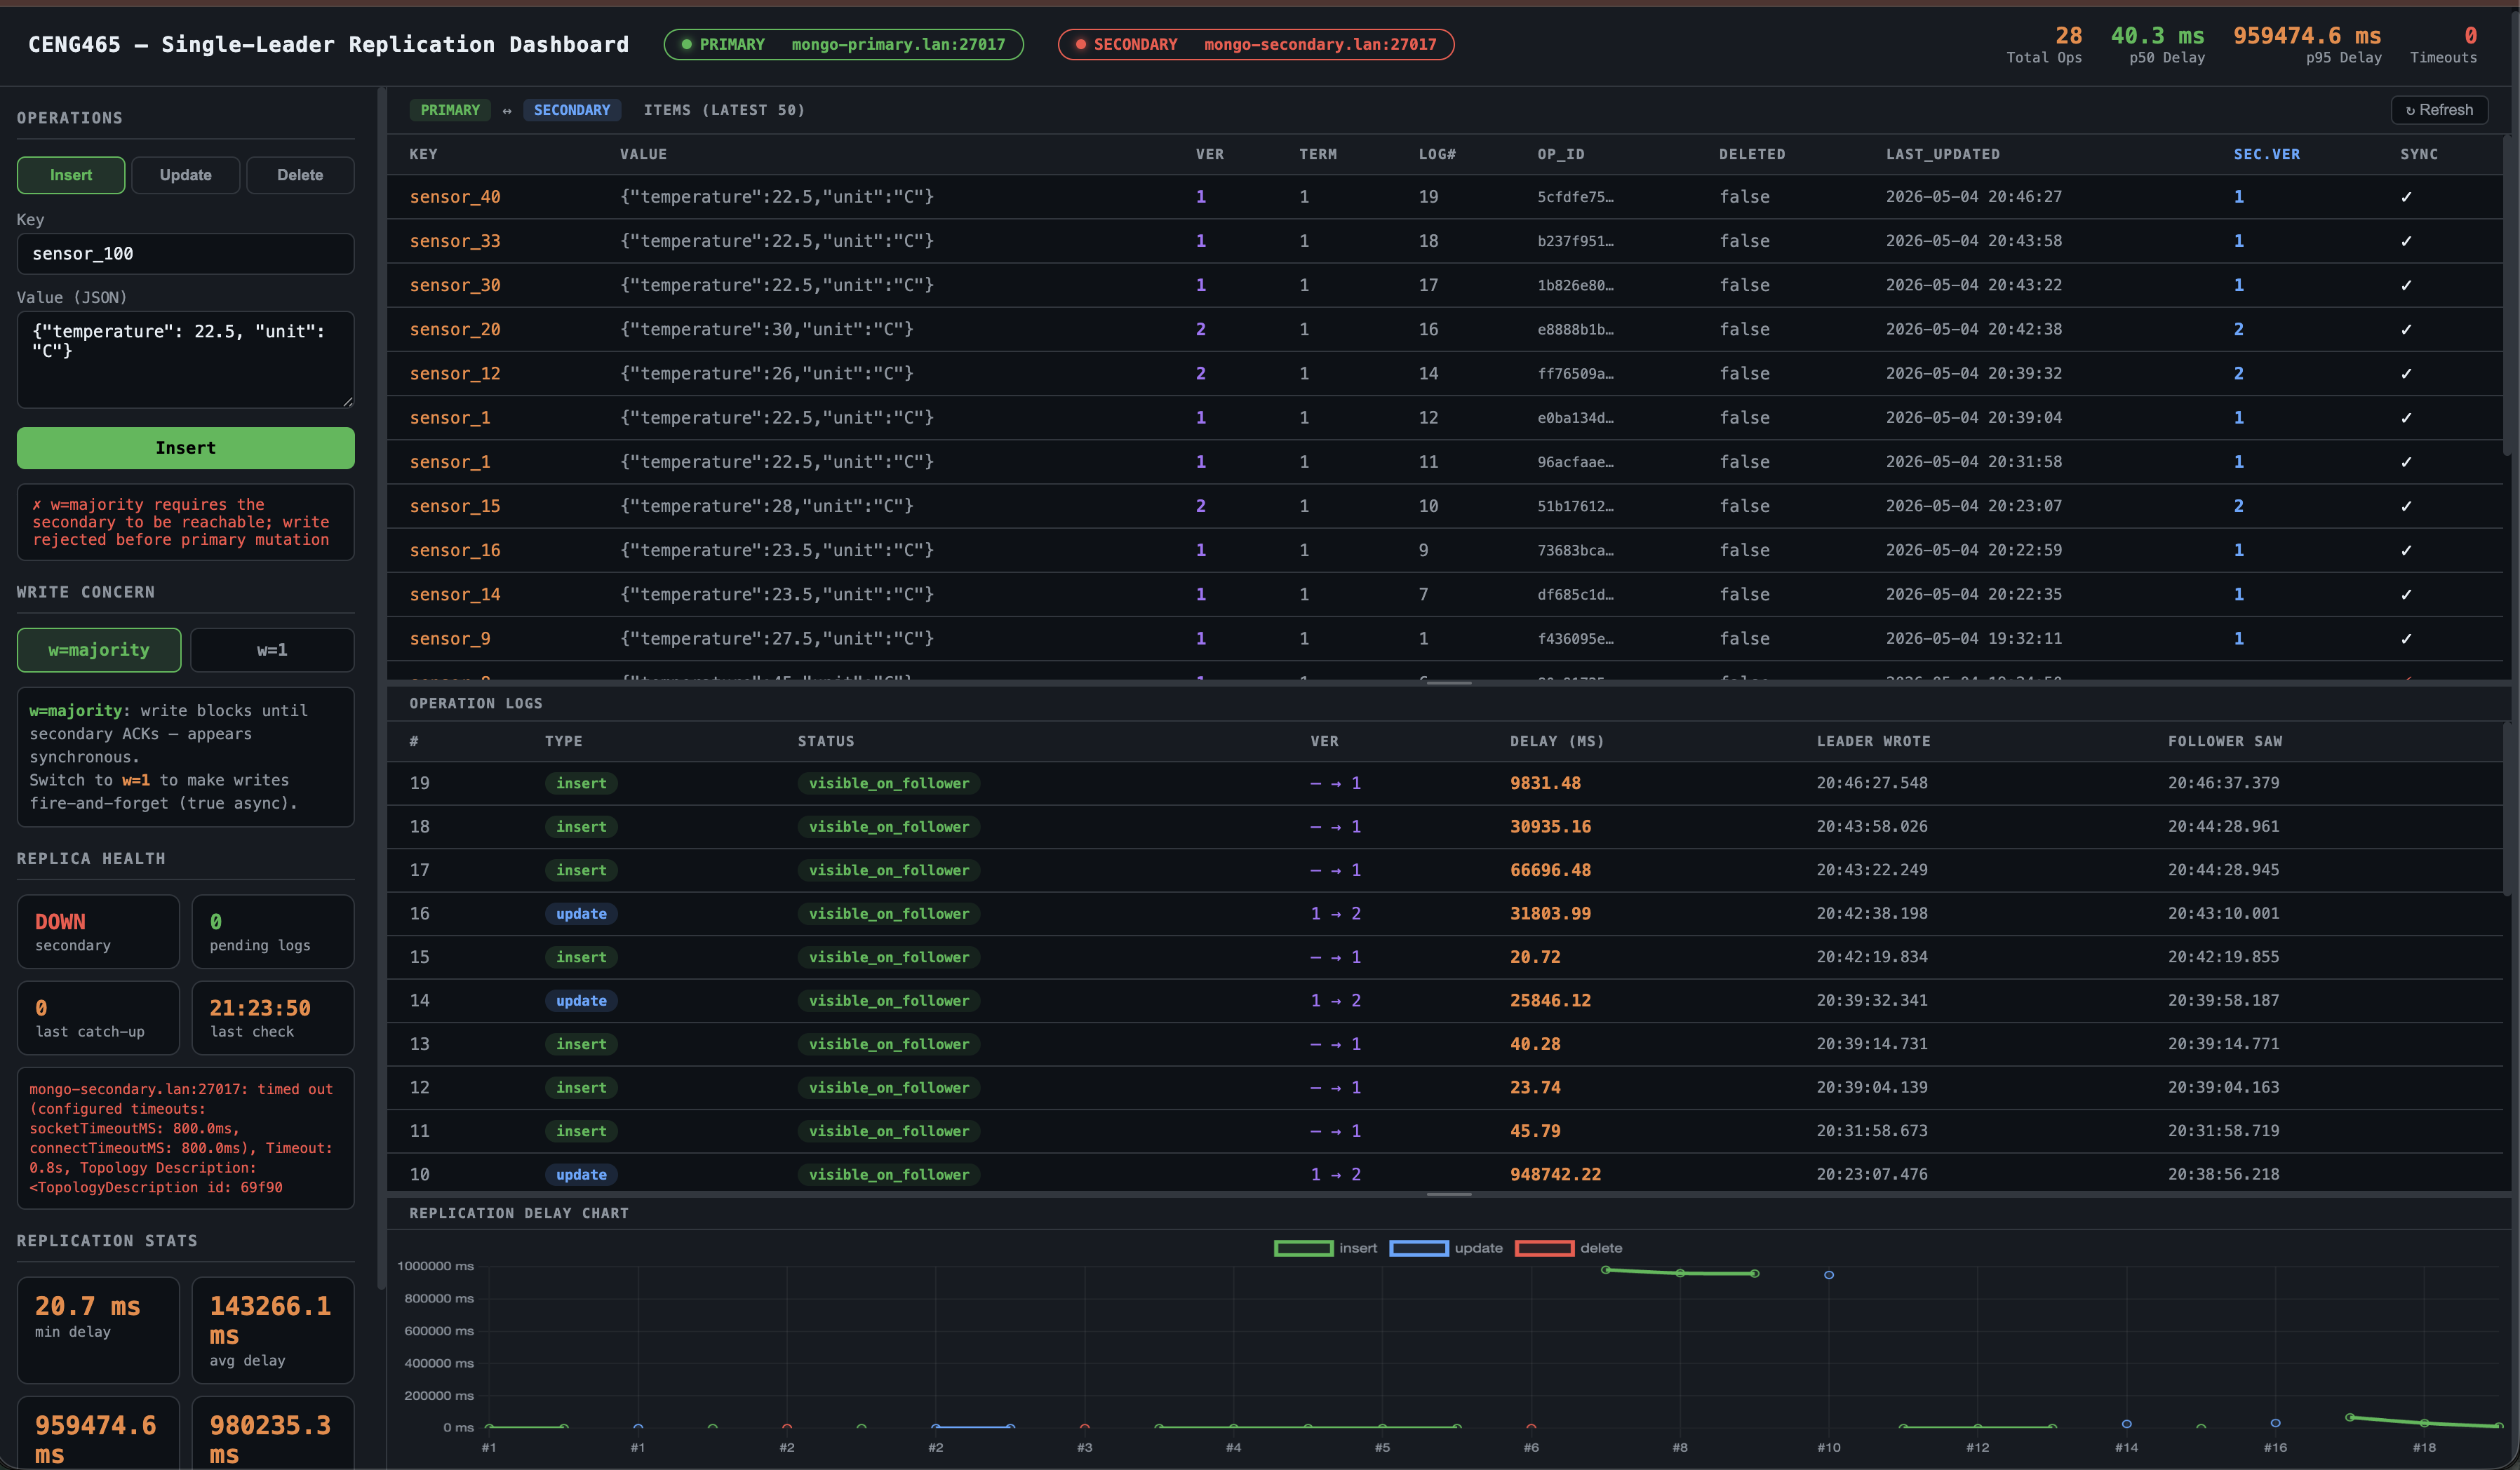
\includegraphics[width=0.92\textwidth,height=0.72\textheight,keepaspectratio]{down_insert_after_majority.png}
  \end{center}
  \begin{center}
    \small Secondary offline. Insert \textcolor{danger}{\textbf{rejected before primary mutation}} — no new item, no pending log created.
  \end{center}
\end{frame}

% ── 8: w=1 Succeeds ───────────────────────────────────────────────────────────
\begin{frame}{Demo Step 2 --- \texttt{w=1} Write Succeeds}
  \begin{center}
    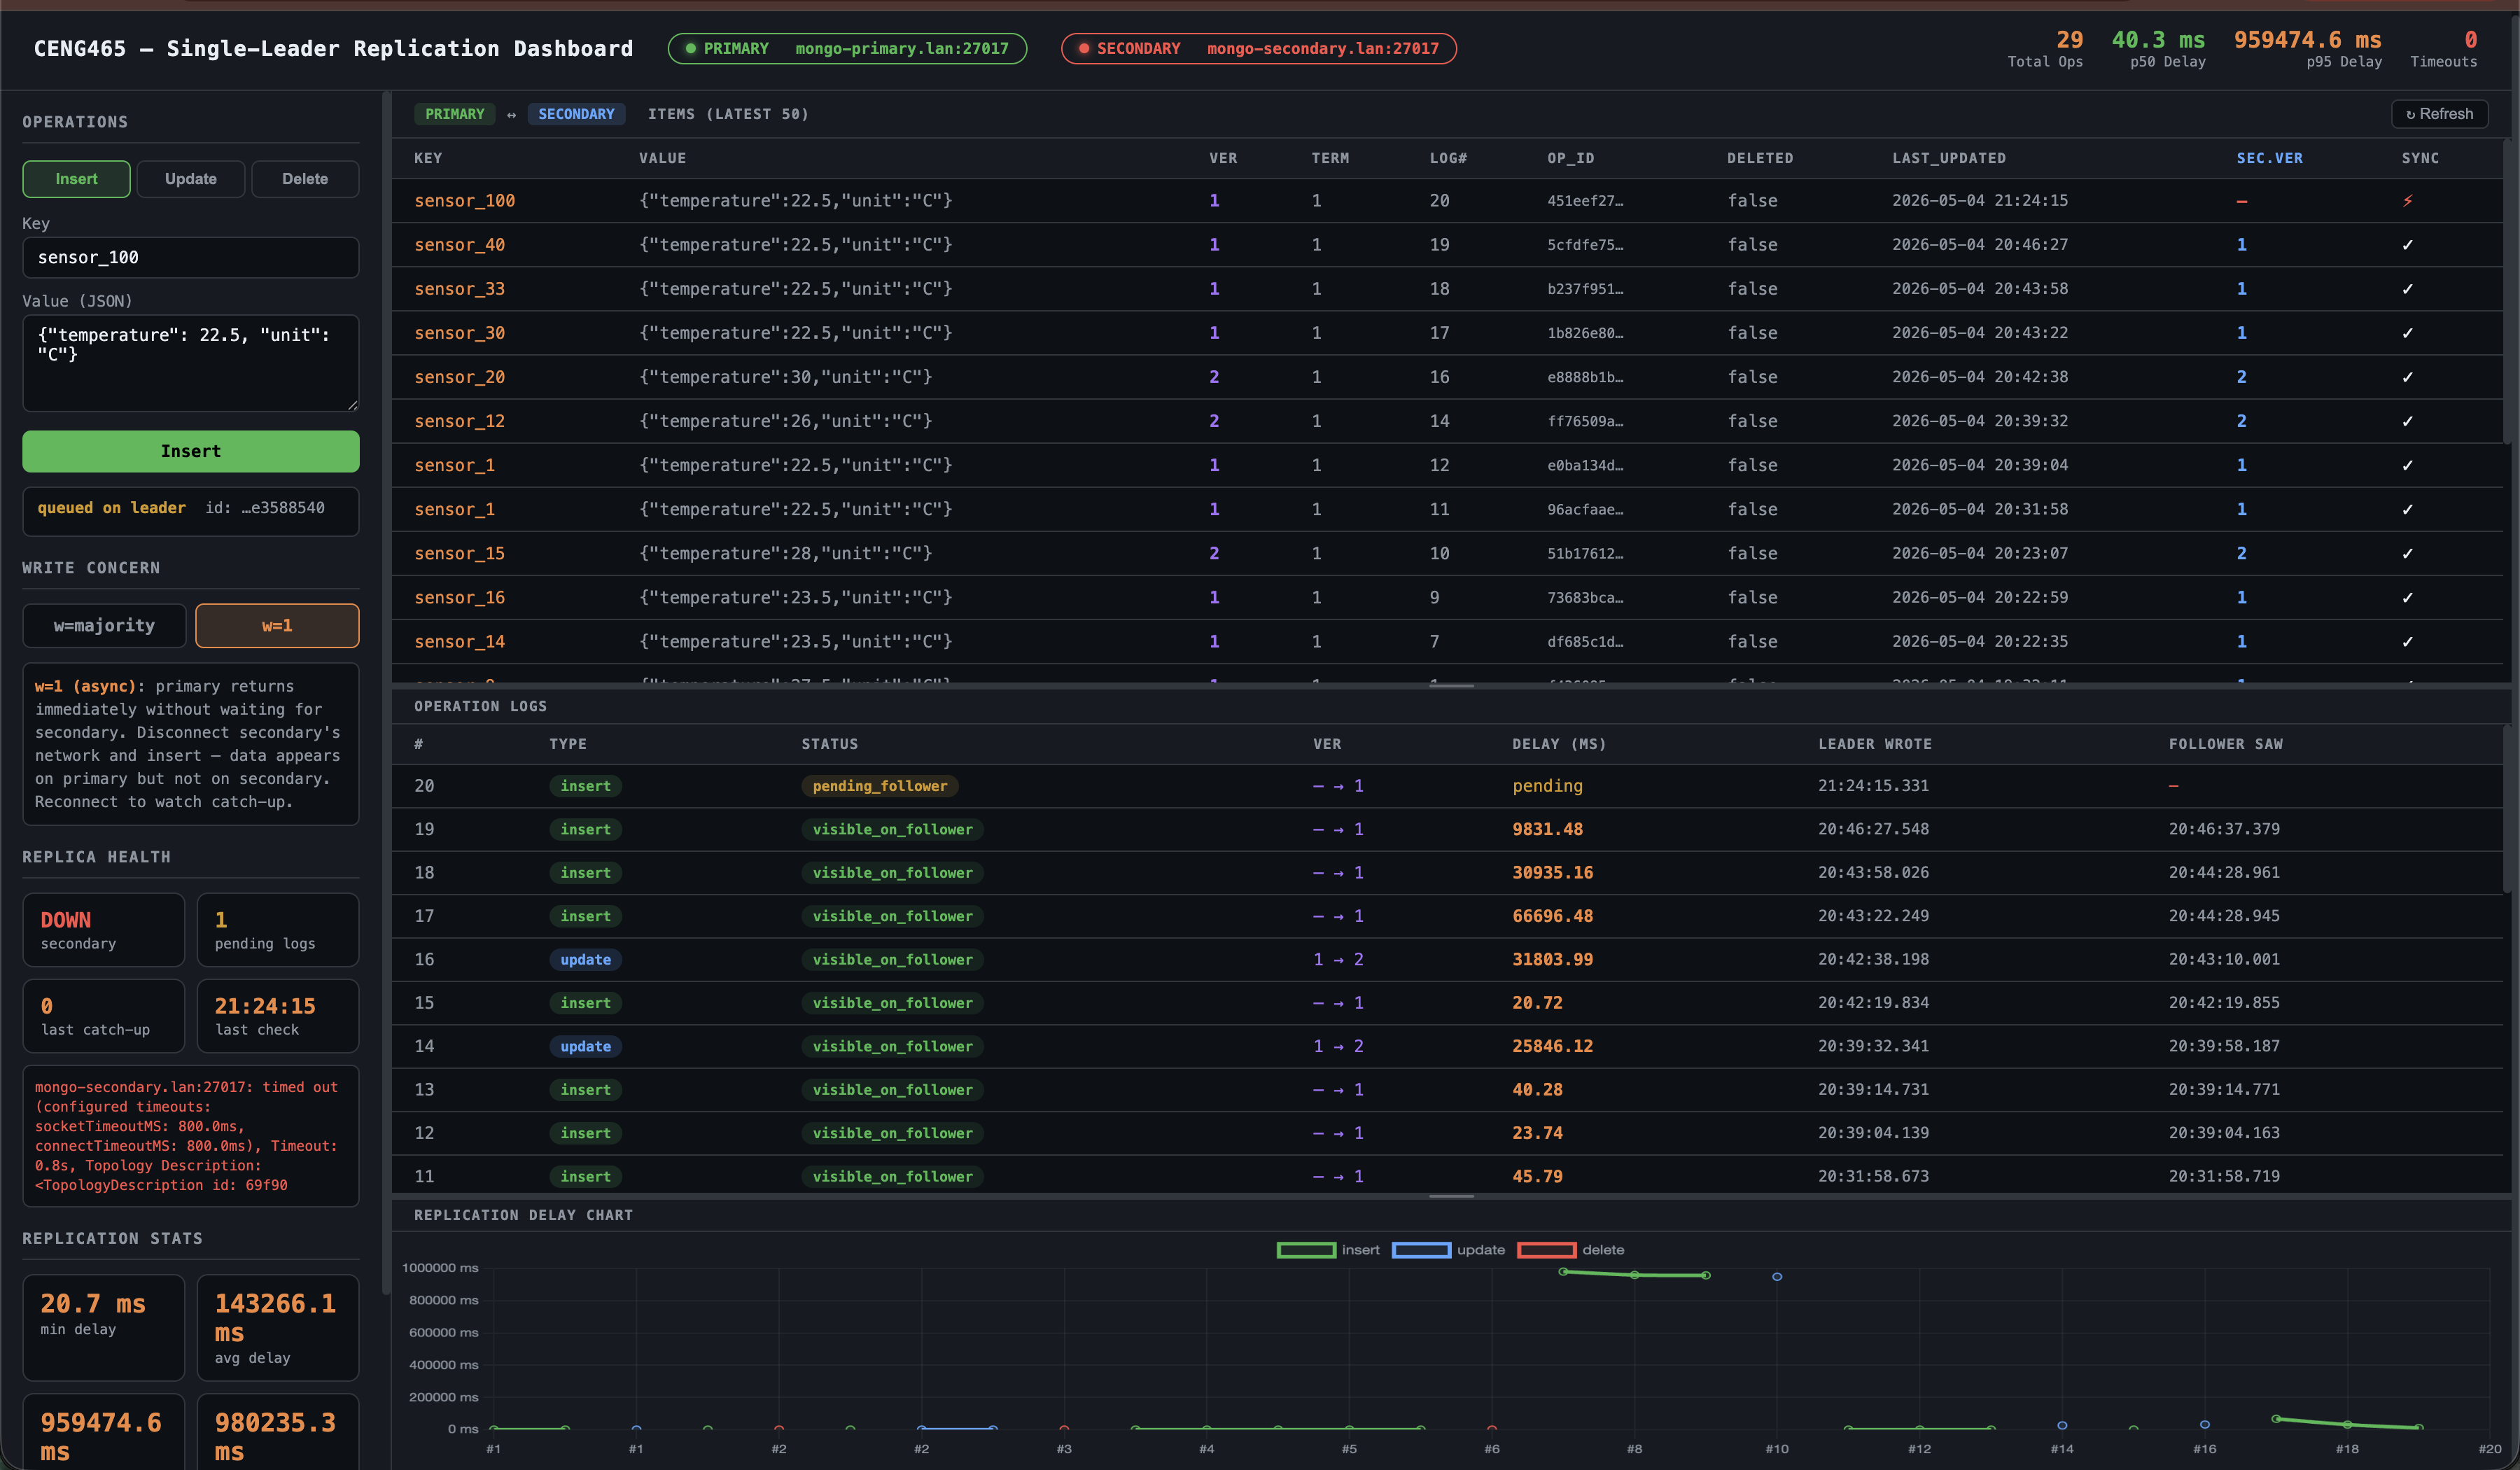
\includegraphics[width=0.92\textwidth,height=0.72\textheight,keepaspectratio]{down_after_inster_w=1.png}
  \end{center}
  \begin{center}
    \small Switched to \texttt{w=1}. Insert completes instantly: \texttt{sensor\_100} on primary (\texttt{ver=1}), \texttt{sec.ver = ---}. Log: \texttt{pending\_follower}.
  \end{center}
\end{frame}

% ── 9: Recovery ───────────────────────────────────────────────────────────────
\begin{frame}{Demo Step 3 --- Secondary Reconnects \& Catches Up}
  \begin{center}
    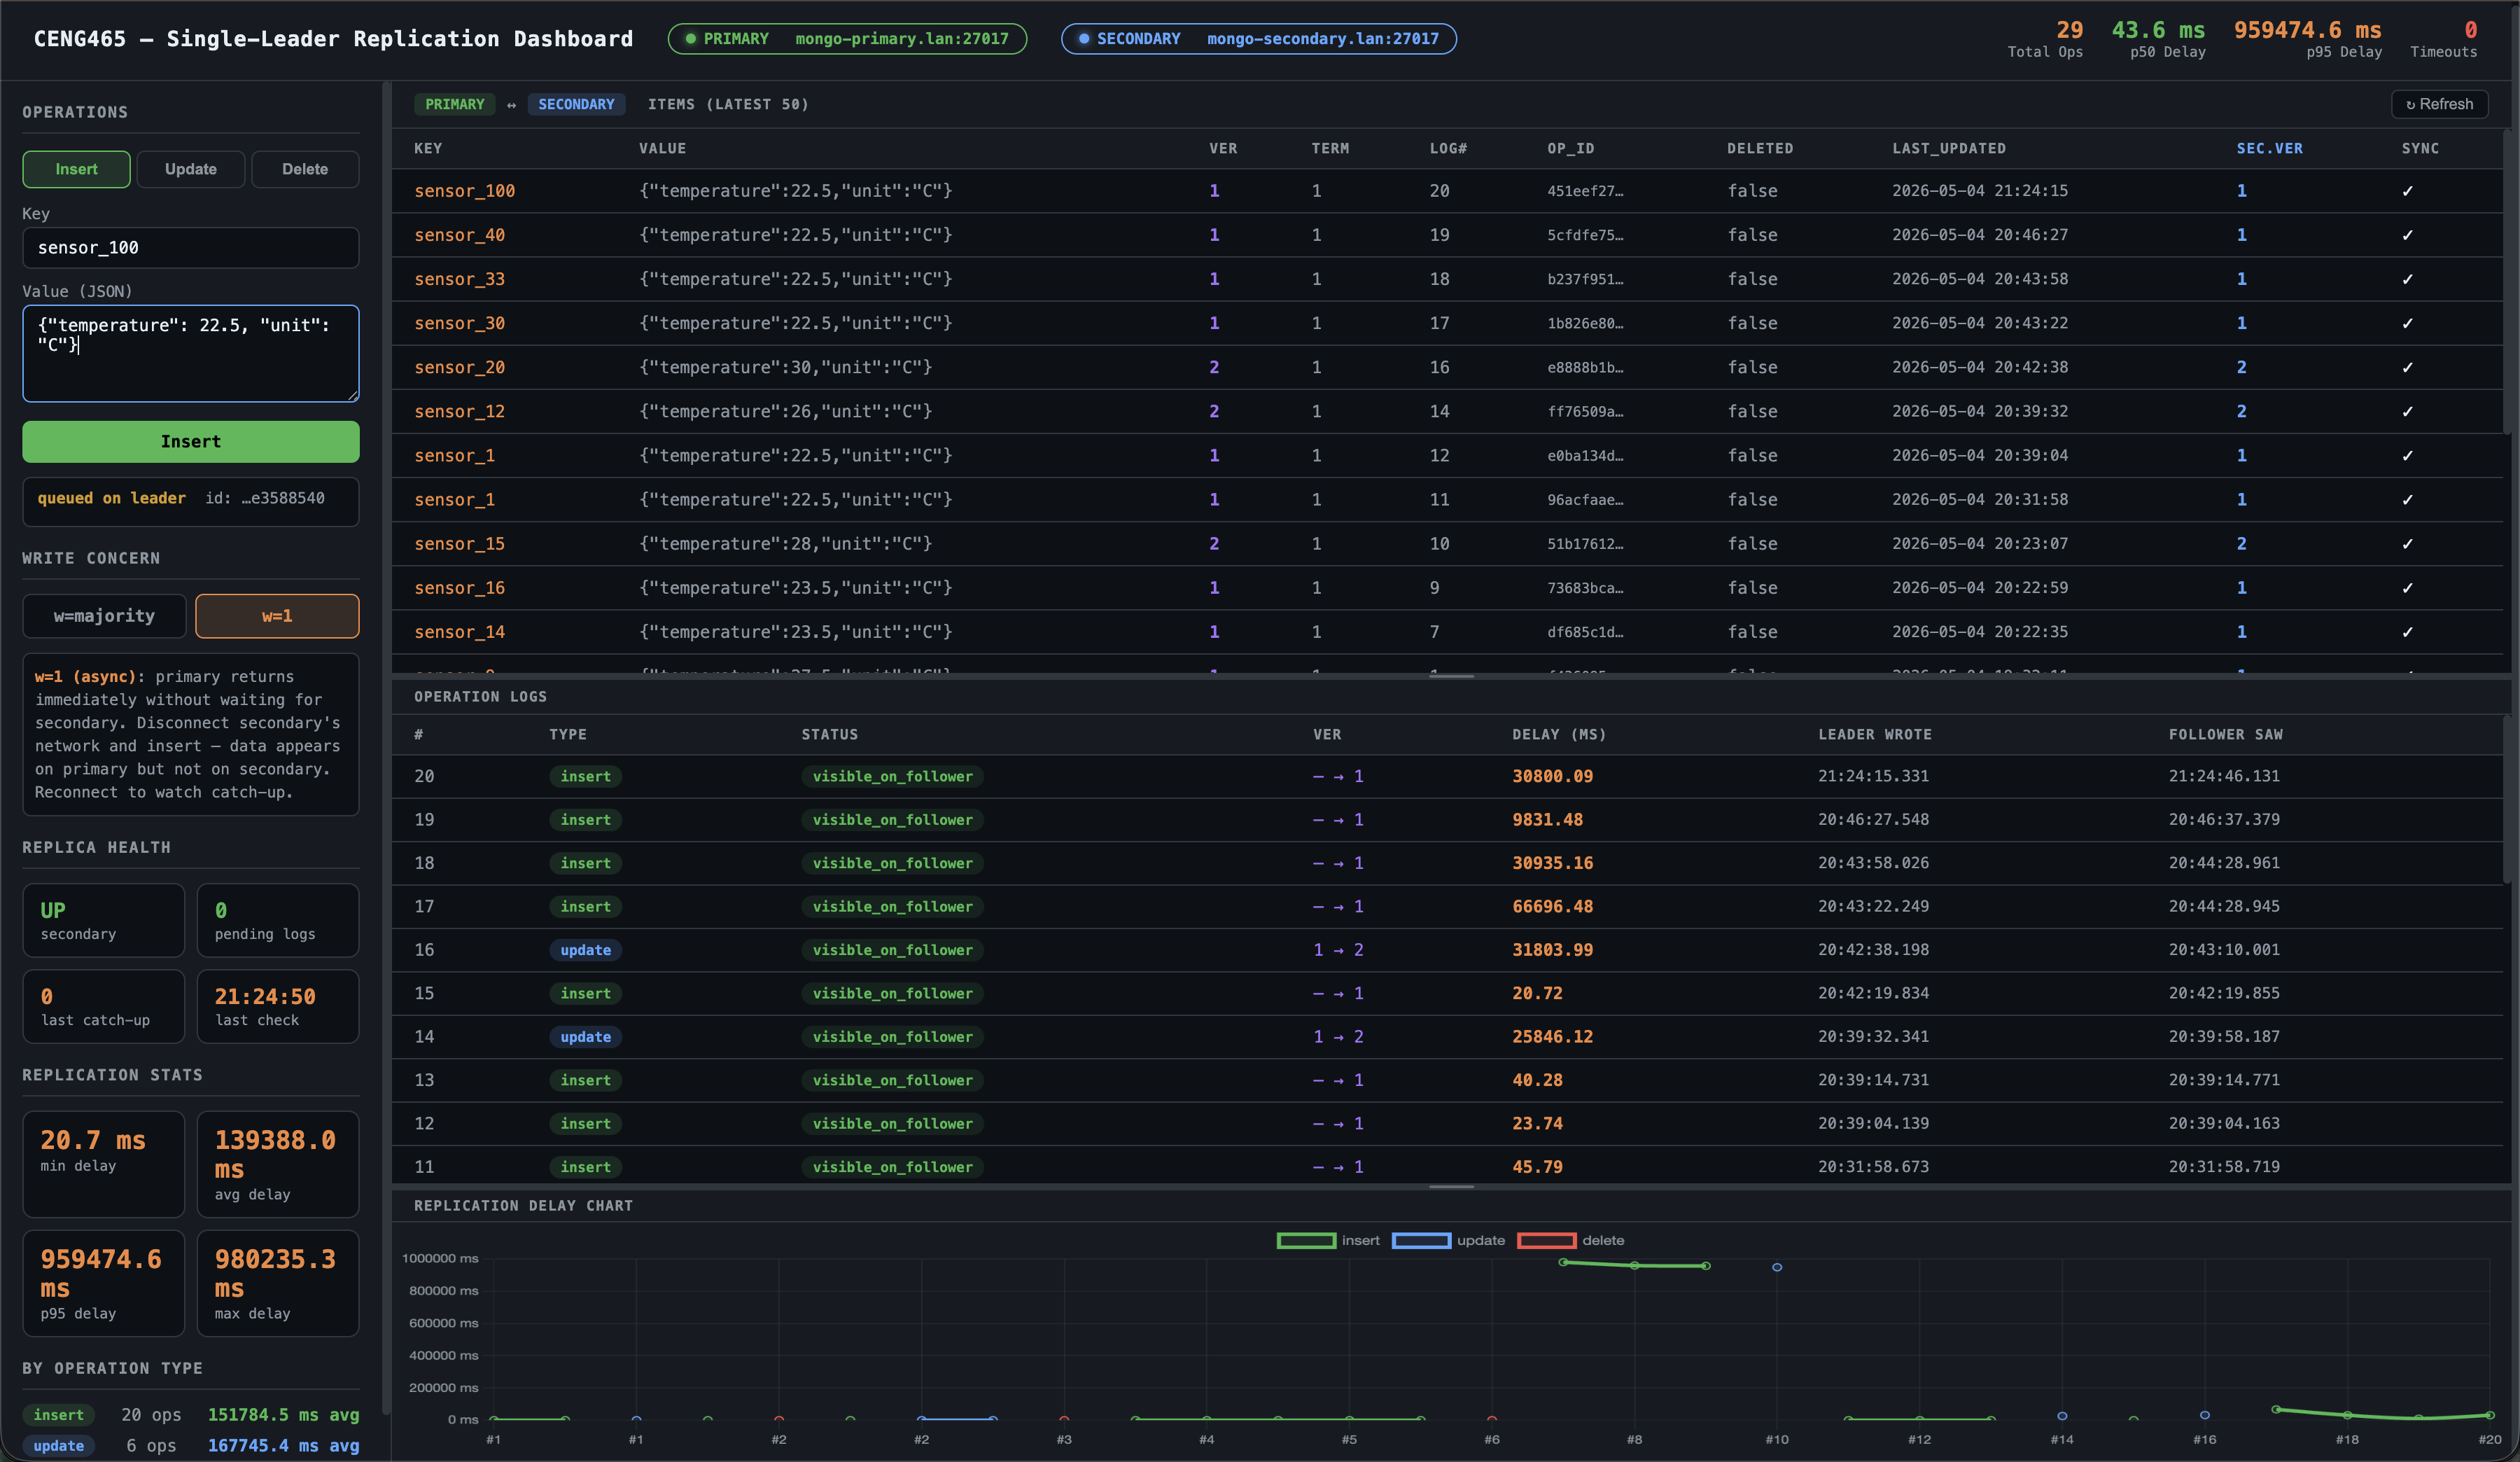
\includegraphics[width=0.92\textwidth,height=0.72\textheight,keepaspectratio]{up_after_down_majority_insert.png}
  \end{center}
  \begin{center}
    \small Oplog replayed; reconciler detects version match. Log: \texttt{visible\_on\_follower}; \texttt{sec.ver} matches; sync \checkmark\ restored.
  \end{center}
\end{frame}

% ── 10: Conclusion ────────────────────────────────────────────────────────────
\begin{frame}{Conclusion}
  \begin{columns}
    \column{0.5\textwidth}
      \small\textbf{What we proved}
      \begin{itemize}\small
        \item Replication is \textbf{asynchronous by default}
        \item Write concern controls the \textbf{durability--availability tradeoff}
        \item \texttt{w=majority}: consistency over availability
        \item \texttt{w=1}: availability with eventual catch-up via oplog
        \item \textbf{Observability} (version, delay, log-index) is essential
      \end{itemize}
    \column{0.46\textwidth}
      \begin{block}{Implementation highlights}
        \footnotesize
        \begin{itemize}
          \item Application-level write guard for \texttt{w=majority}
          \item Background reconciler (1 s cadence)
          \item \texttt{directConnection=true} for honest secondary health
          \item Version + log-index fallbacks for catch-up detection
        \end{itemize}
      \end{block}
      \begin{alertblock}{Key insight}
        \footnotesize Single-leader replication gives strong write ordering but does \textbf{not} guarantee read-after-write consistency on followers.
      \end{alertblock}
  \end{columns}
\end{frame}

\end{document}
